\section{Training Model} \label{sec:build3} Machine Learning models have previously worked wonders on the correct recognition of various algorithms when features extracted are fed into the model for it to figure out the false and the true cases. 

\begin{figure}[t]
	\DeclareGraphicsExtensions{.pdf,.png,.jpg}
	\begin{center}
		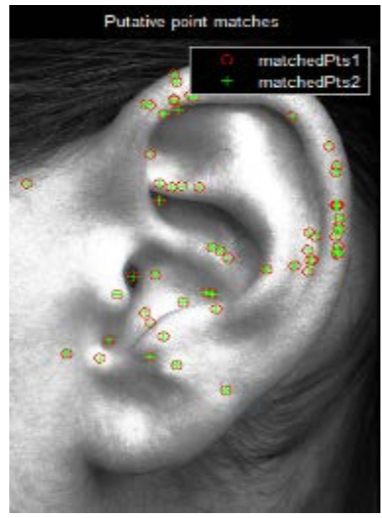
\includegraphics[width=0.5\textwidth]{Figures/Figure15}
	\end{center}
	\caption{The matching results of SURF detector}
	\label{fig:Figure15}
\end{figure}

\begin{figure}[t]
	\DeclareGraphicsExtensions{.pdf,.png,.jpg}
	\begin{center}
		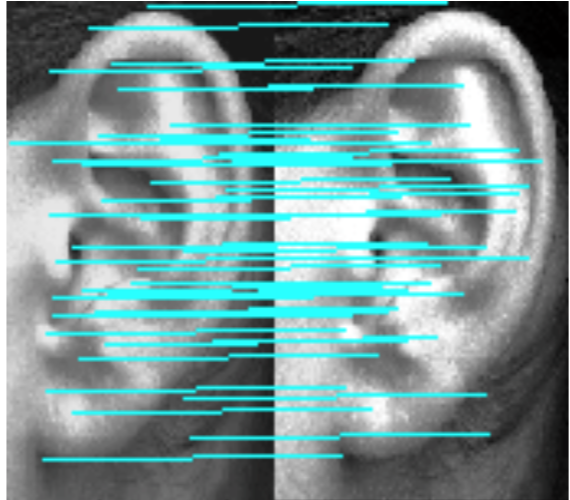
\includegraphics[width=0.5\textwidth]{Figures/Figure16}
	\end{center}
	\caption{The matching results of SIFT detector}
	\label{fig:Figure16}
\end{figure}


\begin{figure}[b]
	\DeclareGraphicsExtensions{.pdf,.png,.jpg}
	\begin{center}
		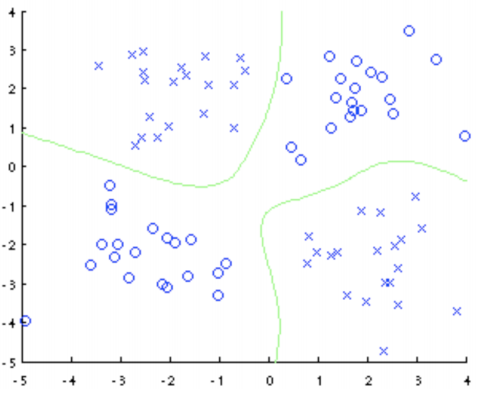
\includegraphics[width=0.5\textwidth]{Figures/Figure10}
	\end{center}
	\caption{Multi-class SVM(from [libSVM paper])}
	\label{fig:Figure10}
\end{figure}


For our purpose we have used Multi-class SVMs. Support Vector Machines were originally designed for binary classification. The formulation to solve Multi-class SVM must have variables which are proportional to the number of different classes. The concept of SVM was proposed by Vapnik [vapnik paper-face recog] et al. They helped to classify almost everything right from linear problems to multi-dimensional problems where the kernel matrix is use to transform the conflicting points into a different dimensional space called the kernel space in order to draw a hyperplane in a conclusive manner so as to separate the different cases. Here multiclass SVM is being used in order to classify the features as extracted by the various feature extraction techniques like SURF and SIFT. After that the model is trained and the features are matched with the features obtained from the query ear image in order to find a nearest match to succeed. Since it is multi-class, thus it helps to create separate classes for different classes of images and helps to classify them when the matching process is being done. The main process of better classification of the model depends on the input features. So as a matter of fact we can say that better the feature extraction is being done, better will be the classification made by the multiclass SVM and thus better will be the results.

The Results can be found in chapter\ref{sec:results}.

